\documentclass{beamer}
\usepackage{physics}
\usepackage{wrapfig}
\usepackage{tikz}
\usepackage{circuitikz}
\usepackage{amsmath}
\usepackage{caption}

\usetikzlibrary{quantikz}

\graphicspath{{./image/}}

\usetheme{default}

\title{Le hack du millenaire?}
\subtitle{Et si on cassait RSA?}
\author{Kwame Yamgnane - kw@qwasar.io - https://github.com/Kwame42/crypto-post-quantum-conference}
\institute{Qwasar Silicon Valley}

\begin{document}


\begin{frame}
        \titlepage
\end{frame}

\begin{frame}{Un processeur}{Transitors}
  \begin{columns}
    \begin{column}{0.5\textwidth}
      PNP
      \begin{circuitikz}
        \draw (0,0) node[pnp] (pnp) {};
      \end{circuitikz}
    \end{column}
    \begin{column}{0.5\textwidth}
      NPN
      \begin{circuitikz}
        \draw (0,0) node[npn] (npn) {};
      \end{circuitikz}
    \end{column}
  \end{columns}
\end{frame}

\begin{frame}{Un processeur}{Portes logiques = groupe de transistor / NAND}
  \begin{columns}
    \begin{column}{0.5\textwidth}
      \begin{circuitikz}
        \draw (0,2) node[npn](p1){};
        \draw (0,0) node[npn](p2){};
        \draw (-2,6) node[pnp](n1){};
        \draw (0,4) node[pnp](n2){};
        \draw (p1.E) -- (p2.C);
        \draw (p2.B) |- (n2.B);
        \draw (n1.B) |- (p1.B);
        \draw (n1.C) |- (n2.C);
        \draw (n2.C) to [short, *-o] ++(1.5,0);
        \draw (n1.E) to [short, -o] ++(3.5,0);
        \draw (n2.E) to [short, -*] ++(0,2);
        \draw (p2.E) to [short, -o] ++(1.5,0);
        \draw (p1.C) to (n2.C);
        \draw (-3.5,1.5) to[short, o-*] (-0.84,1.5);
        \draw (-3.5,4) to[short, o-*] (-2.84,4);
        \draw node [left] at (-3.5, 4) {A};
        \draw node [left] at (-3.5, 1.5) {B};
        \draw node [above] at (1.25, 6) {0};
        \draw node [below] at (1.25, 4) {out};
        \draw node [below] at (1.25, 0) {1};
      \end{circuitikz}
    \end{column}
    \begin{column}{0.25\textwidth}
      \begin{table}
        \begin{tabular}{r|c|c}
          A & B & Out  \\ \hline
          0 & 0 & 1 \\
          1 & 0 & 0 \\
          0 & 1 & 0 \\
          1 & 1 & 0 \\
        \end{tabular}
        \caption{NAND}
      \end{table}
    \end{column}
    \begin{column}{0.25\textwidth}
      \begin{circuitikz}
        \draw (0,0) node[nand port] {};
      \end{circuitikz}
    \end{column}
  \end{columns}
\end{frame}

\begin{frame}{Les portes logiques}{le binaire: l'addition (NDLR: je sais y a pas le retenu on fera a l'oral :D)}
  \begin{columns}
    \begin{column}{0.3\textwidth}
      \begin{table}
        \begin{tabular}{c|c}
          0 & 0 0 0  \\ \hline
          \color{blue}1 & \color{blue}0 0 1  \\ \hline
          \color{cyan}2 & \color{cyan}0 1 0  \\ \hline
          \color{red}3 & \color{red}0 1 1  \\ \hline
          ... &... \\ \hline
          7 & 1 1 1  \\ \hline
        \end{tabular}
        \caption{3 bit integer}
      \end{table}
    \end{column}
    \begin{column}{0.3\textwidth}
      \begin{table}
        \begin{tabular}{r|c|c}
          A & B & Out  \\ \hline
          0 & 0 & 0 \\
          1 & 0 & 1 \\
          0 & 1 & 1 \\
          1 & 1 & 1 \\
        \end{tabular}
        \caption{OR}
      \end{table}
    \end{column}
    \begin{column}{0.3\textwidth}
      \begin{circuitikz}
        \draw (0,0) node[or port] {2};
        \draw (0,2) node[or port] {1};
        \draw (0,4) node[or port] {0};
        \draw node [above] at (-1.75, 4) {\color{blue}$1_1$};
        \draw node [below] at (-1.75, 4) {\color{cyan}$0_2$};
        \draw node [above] at (-1.75, 2) {\color{blue}$0_1$};
        \draw node [below] at (-1.75, 2) {\color{cyan}$1_2$};
        \draw node [above] at (-1.75, 0) {\color{blue}$0_1$};
        \draw node [below] at (-1.75, 0) {\color{cyan}$0_2$};
        \draw node [] at (0.5, 4) {\color{red}$1_3$};
        \draw node [] at (0.5, 2) {\color{red}$1_3$};
        \draw node [] at (0.5, 0) {\color{red}$0_3$};
      \end{circuitikz}
    \end{column}
  \end{columns}
\end{frame}

\begin{frame}{Complexite des Algorithmes}
  \begin{columns}
    \begin{column}{0.5\textwidth}
      \begin{itemize}
      \item Algorithmes compliqu\'{e}s
        \color{red}
      \item Algorithmes NP : Compliqu\'{e}s \`a executer, facile \`a r\'esoudre
        \color{blue}
      \item Algorithmes P : faciles \`a executer et \`a resoudre
      \end{itemize}
    \end{column}
  
    \begin{column}{0.5\textwidth}
      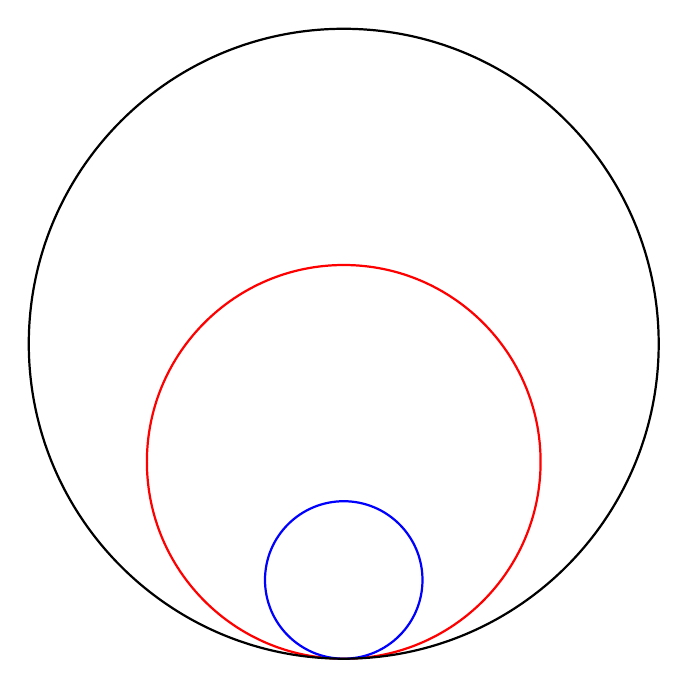
\begin{tikzpicture}
        \draw[thick, red] (2,2) circle (2.5cm);
        \draw[thick, blue] (2,0.5) circle (1cm);
        \draw[thick] (2,3.5) circle (4cm);
      \end{tikzpicture}
    \end{column}
  \end{columns}
\end{frame}

\begin{frame}{Algorithmes NP}{Exemple}
  \begin{columns}
    \begin{column}{0.5\textwidth}
      \begin{itemize}
      \item Trouver les facteurs premiers de $82661 \leftarrow NP$
      \item $41x43x47 = 82661 \leftarrow P$
      \end{itemize}
    \end{column}
    
    \begin{column}{0.5\textwidth}
      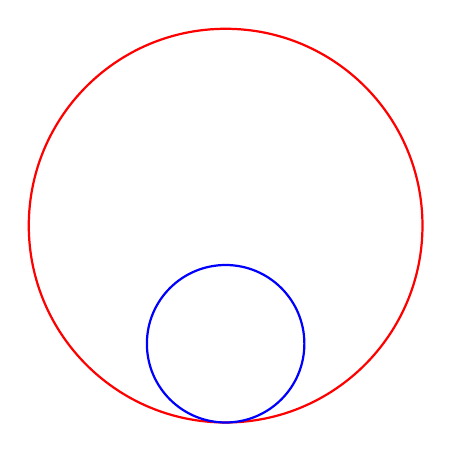
\begin{tikzpicture}
        \draw[thick, red] (2,2) circle (2.5cm);
        \draw[thick, blue] (2,0.5) circle (1cm);
      \end{tikzpicture}
    \end{column}
  \end{columns}
\end{frame}

\begin{frame}{P = NP... }{... ou qui veut gagner 1 million ?}
  \begin{columns}
    \begin{column}{0.5\textwidth}
      Les algorithmes de crypto sont NP
    \end{column}
    
    \begin{column}{0.5\textwidth}
      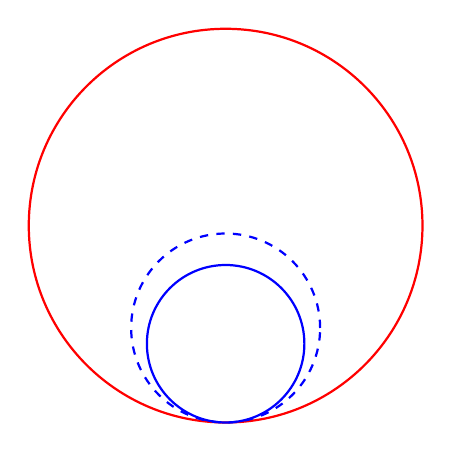
\begin{tikzpicture}
        \draw[thick, red] (2,2) circle (2.5cm);
        \draw[thick, blue, dashed] (2,0.70) circle (1.2cm);
        \draw[thick, blue] (2,0.5) circle (1cm);
      \end{tikzpicture}
    \end{column}
  \end{columns}
\end{frame}

\begin{frame}{Quelques bases}{La m\'{e}canique quantique}
  \begin{center}
    \begin{tabular}{ c c c }
      Le tout petit & \`{A} l'echelle humaine  & \`{A} partir de 1 \(M_\odot\) \\
      (niveau Atom) & & \\
      \includegraphics[height=2cm]{Atome_lithium_rutherford.png} & \includegraphics[height=2cm]{TerreWorldWind.jpg} & \includegraphics[height=2cm]{04-965413833409_COI.jpeg}\\
      Mecanique Quantique & Newton & Relativite generale \\
       &  & Newton Etendu \\
    \end{tabular}
  \end{center}
\end{frame}

\begin{frame}{Superposition Quantique}{``je suis inombrable''}
  \begin{center}
    \includegraphics[width=9cm]{3604843-inline.jpg}\\
    \vspace{0.5cm}
    $\ket{\Psi} = a \ket{Jeune} + b \ket{Agee}$ 
  \end{center}
\end{frame}

\begin{frame}{Intrication Quantique}{``L'espace et le temps n'existent pas''}
  \begin{center}
        \includegraphics[width=9cm]{intrication.png}\\
    \vspace{0.5cm}
    $\ket{\Psi(v1, v2)} = \frac{1}{\sqrt{2}}(\ket{\Psi(\uparrow\downarrow)} - \ket{\Psi(\downarrow\uparrow)})$
  \end{center}
\end{frame}

\begin{frame}{le Q Bit}
  Etat propre...
  \begin{equation*}
    \ket{0} =
    \begin{bmatrix}
      1 \\
      0 
    \end{bmatrix}
  \end{equation*}
  ...ou par exemple
  \begin{equation*}
    \ket{1} =
    \begin{bmatrix}
      0 \\
      1 
    \end{bmatrix}
  \end{equation*}
    Mais aussi ...
  \begin{equation*}
    50\%\ket{0} + 50\%\ket{1} =
    \begin{bmatrix}
      0.5 \\
      0.5 
    \end{bmatrix}
  \end{equation*}
\end{frame}

\begin{frame}{Les portes logiques quantiques}
  \begin{columns}
    \begin{column}{0.25\textwidth}
      \begin{center}
        \begin{circuitikz}[scale=0.8, transform shape]
          \draw (0,0) node[not port] {};
        \end{circuitikz}
        \begin{table}
          \begin{tabular}{r|c|c}
            A & NOT A \\ \hline
            0 & 1 \\
            1 & 0 \\
          \end{tabular}
        \end{table}
      \end{center}
    \end{column}
    \begin{column}{0.75\textwidth}
      \begin{center}
        \begin{quantikz}
          \gate{X}\\
        \end{quantikz}
        \begin{equation*}
          \begin{bmatrix}
            \color{red}0 & \color{blue}1\\
            \color{cyan}1 & \color{green}0
          \end{bmatrix}
          \begin{bmatrix}
            1\\
            0
          \end{bmatrix}
          =
          \begin{bmatrix}
            \color{red}0 \color{black}\times1 + \color{blue}1 \color{black}\times0\\
            \color{cyan}1 \color{black}\times1 + \color{green}0 \color{black}\times0
          \end{bmatrix}
          =
          \begin{bmatrix}
            0\\
            1
          \end{bmatrix}
        \end{equation*}
      \end{center}
    \end{column}
  \end{columns}
\end{frame}

\begin{frame}{Capacite de calcul}{Registre ?}
  \begin{columns}
    \begin{column}{0.25\textwidth}
      \begin{table}
        \begin{tabular}{ll}
          1 & 000\\
          2 & 001\\
          3 & 010\\
          4 & 011\\
          5 & 100\\
          6 & 101\\
          7 & 110\\
          8 & 111\\
        \end{tabular}
      \end{table}
    \end{column}
    \begin{column}{0.75\textwidth}
      \begin{table}
        $2^3 = 8$
        \begin{tabular}{l}
          $10\%\ket{000}+8\%\ket{001}+12\%\ket{010}+5\%\ket{011}$\\
          $+10\%\ket{100}+20\%\ket{101}+5\%\ket{110}+30\%\ket{111}$\\
        \end{tabular}
      \end{table}
      \begin{itemize}
      \item attention 1 seule reponse possible !
      \item Integer, registre de 64 bit 
      \item soit en Qbits $2^{64} = 1.8x10^{19}$ fois plus rapide...
      \item Mais on peut aussi faire des Qtrits : $3^{64} = 3.4x10^{30}$
      \end{itemize}
    \end{column}
  \end{columns}
\end{frame}

\begin{frame}{Algorithme de SHOR}{}
  \includegraphics[height=5cm]{shor.png}
  \begin{itemize}
  \item 2000 Qbit 
  \item $10^9$ Qbit avec code d'erreur...
  \end{itemize}
\end{frame}

\begin{frame}{Ordinateur quantique}{Avec Google tout va plus vite :D }
  \begin{center}
    \includegraphics[height=3cm]{sycamore1.jpeg}
    \includegraphics[height=3cm]{sycamore2.png}
  \end{center}
  \begin{itemize}
  \item Google processeur Sycamore : 53 Qbit
  \item Supremacie Quantique : 200s (53) vs 10,000 ans (1,000,000 de coeur)
  \item Un algo qui ne sert a rien :D
  \end{itemize}
\end{frame}

\begin{frame}{Alors qu'es ce qui tiens ?}
  Creation de nouveaux algorithmes de securites \footnote{liste non exhaustive... meme si c'est le titre de la conference c'etait un pretexte pour vous presenter les ordi...}
  \begin{itemize}
    \item Clef publiques :
      \begin{enumerate}
      \item \href{https://pq-crystals.org/}{CRYSTALS-KYBER} : clef publiques
      \end{enumerate}
    \item Signature electronnique :
      \begin{enumerate}
      \item \href{https://pq-crystals.org/}{CRYSTALS-DILITHIUM} : clef publiques
      \item \href{https://pq-crystals.org/}{FALCON} : clef publiques
      \end{enumerate}
  \end{itemize}
\end{frame}

\begin{frame}{Il faut s'en occcuper}{meme si ce n'est pas pour tout de suite}
  \begin{center}
    \begin{figure}
      \includegraphics[height=7cm]{eth.jpg}
      \caption*{Credit photo: Mathias Herberts ETHCC[5] -- July 2022}
    \end{figure}
  \end{center}
\end{frame}

\begin{frame}
        Merci !
\end{frame}

\begin{frame}{Exhibit}{Les conferences d'Alain Aspect}

\end{frame}

\begin{frame}{Exhibit}{La chaine youtue de David Louarpe Science Etonnante}
  \begin{description}
  \item \href{https://www.youtube.com/watch?v=Rj3jTw2DxXQ&t=3s}{La mécanique quantique en 7 idées}
  \item \href{https://www.youtube.com/watch?v=5R6k2mEacZo&t=8s}{L'intrication quantique}
  \item \href{https://www.youtube.com/watch?v=hB1kmGzpIrw}{Les expériences d'Alain ASPECT}
  \item \href{https://www.youtube.com/watch?v=OeZ_63iKPho&t=556s}{Alain Aspect : Interview complète}
  \item \href{https://www.youtube.com/watch?v=hB1kmGzpIrw}{Le mystère des gâteaux quantiques}
  \item \href{https://www.youtube.com/watch?v=KaRd_eB2qOA}{La Suprématie Quantique de Google}
  \item \href{https://www.youtube.com/watch?v=AgtOCNCejQ8}{P = NP}
  \end{description}
\end{frame}

\begin{frame}{Exhibit}{Disclaimer}
  \begin{description}
  \item Speakable and Unspeakable in Quantum Mechanics: Collected Papers on Quantum Philosophy
  \item L'Impensable Hasard: Non-localité, téléportation et autres merveilles quantiques
  \item Introduction to Quantum Optics: From the Semi-classical Approach to Quantized Light
  \end{description}
\end{frame}

\end{document}
